% !TEX TS-program = pdflatex
% !TEX encoding = UTF-8 Unicode

\documentclass{beamer}

\usepackage[english]{babel}

\usepackage[utf8]{inputenc}

\usepackage{times}
\usepackage[T1]{fontenc}

\usepackage{csquotes}

\usepackage{tikz}
\usetikzlibrary{decorations.pathreplacing,calc,tikzmark}

\title[]{Principles of methodology of science}

%\subtitle
%{} % (optional)

\author[] % (optional)
{Agent c2b1e19611723c8a807351d4bde59bf27a68488b}

\institute[Independent (no affiliation)] % (optional)
{
Independent (no affiliation)
}
% Use the \inst command if there are several affiliations.

\date[\today] % (optional)
{\today}

\subject{}
% inserted into the PDF information catalog. 

% can add a logo (e.g. university) as follows:

% \pgfdeclareimage[height=0.5cm]{university-logo}{university-logo-filename}
% \logo{\pgfuseimage{university-logo}}

% step-wise
%\beamerdefaultoverlayspecification{<+->}



\begin{document}

\begin{frame}
  \titlepage
\end{frame}

\begin{frame}

%\begin{quotation}
\enquote{Estaba ya próximo el dia destinado para aparecer el hombre sobre la tierra y mostrarse á la luz del sol, y Prometeo no sabia qué hacer, para dar al hombre los medios de conservarse. En fin, hé aquí el expediente á que recurrió: robó á Vulcano y á Minerva el secreto de las artes y el fuego, porque sin el fuego las ciencias no podian poseerse y serian inútiles, y de todo hizo un presente al hombre. Hé aquí de qué manera el hombre recibió la ciencia de conservar su vida; pero no recibió el conocimiento de la política, porque la política estaba en poder de Júpiter, y Prometeo no tenia aún la libertad...}
%\end{quotation}

\rightline{Protágoras, Diálogos socráticos (Platón)}

\end{frame}

\begin{frame}{Outline}
  \tableofcontents
  % [pausesections]
\end{frame}

\section{Principles and definitions}

\begin{frame}{Principles and definitions}{}
  \begin{itemize}
  \item The material principle.
  \item The plurality of matter principle.
  \item The connectivity principle.
  \item The no universality principle.
  \item Axiom of self-replication.
  \item Axiom of choice.
  \item Axiom of replication.
  \end{itemize}
\end{frame}

\subsection{Minimal principles rationality}

\begin{frame}{Minimal principles of rationality}

\Large A small set of principles that must be necessarily assumed in order to be rational.

\end{frame}

\begin{frame}{The material principle}

\begin{center}
{\Large If something exists it is matter. If something is matter it exists.\\}

It is a fundamental ``negative'' principle against idealism and derivations.
\end{center}

\end{frame}

\begin{frame}{The plurality of matter principle}

\begin{center}
\Large There exist different types of matter, that is, matter is plural, diverse.
\end{center}

\end{frame}

\begin{frame}{The connectivity principle}

\begin{center}
\Large Everything is connected with something and nothing is connected with everything.
\end{center}

\end{frame}

\begin{frame}{The no universality principle}

\begin{center}
{\Large Nothing is universal.}\\
\end{center}

\vspace{1cm}
When we use terms such as ``everything'', ``all'', ``universe'', etc., they must always be interpreted carefully. Either:
\begin{enumerate}
\item Use the term but qualify it referring to a context. For instance, in the context of medicine ``all'' can mean ``all human bodies''. This does not contradict the no universality principle.
\item Use the term only to criticize it as confusing. For instance, when we criticize religion or other dogmatisms.
\end{enumerate}
\end{frame}

\begin{frame}{Axiom of self-replication}

\begin{center}
{\Large Matter tends to preserve itself or, equivalently, to self-replicate across time.\\}
\end{center}

The axiom of self-replication is one of the elemental operations of matter.

\end{frame}

\begin{frame}{Axiom of choice}{}

\begin{center}
{\Large Given a set we say a subset is chosen when the subset is replicated.\\}
\end{center}

The axiom of choice is one of the elemental operations of matter.
  
\end{frame}

\begin{frame}{Axiom of replication}

\begin{center}
{\Large We say an object is replicated when an object self-replicates (axiom of self-replication) and it chooses (axiom of choice) a subset. The subset is the replicated object.}
\end{center}

There is a recursive form in the principles.

\end{frame}


\section{Definition of technique and science}

\begin{frame}{Definition of technique and science}{}
  \begin{itemize}
  \item The essence of science or technique is control, the characteristic is replication or reproduction.
  \item Sciences and techniques, like matter, are plural. There is no such thing as \textit{the} science, or \textit{the} technique.
  \item A technique is a mechanical procedure defined by a set of objects, a set of operations and a replication function/constraint.
  \item A science is, essentially, the same as a technique. This notion will probably be refined later.
  \end{itemize}
\end{frame}


\section{Demarcation criteria: necessary condition for science and technique}

\begin{frame}{Demarcation criteria}{}
  \begin{itemize}
  \item Reproducibility.
  \end{itemize}
\end{frame}

\section{Example: the problematic case of economics}

\begin{frame}{Example: the problematic case of economics}

  \begin{itemize}
  \item What is economics?
  \item Its scientificity is questioned.
   \item Problematic definition of its object.
   	\begin{itemize}
   	\item \textit{The} science of reproduction? Form of monism, contradicts minimal principles of rationality.
   	\item \textit{The} science of exchange? Workaround, but ultimately also contradicts the same principles.
   	\end{itemize}
   \item Lacks characteristic. Not satisfying demarcation criteria. Non reproducibility, predictive power, etc.
   \item Confusion is systematic (original), not coincidental.
  \end{itemize}
\end{frame}

\begin{frame}{Example: the problematic case of economics}

  \begin{itemize}
  \item If economics is something (substantial) at all, then it must be the science of exchange.
  \item Economics is the science of exchanging objects. In order to do that, economics relies on the techniques of coins/currencies.
  \item If a coin is something (substantial) at all, it must be a relationship of equivalence between (potentially) all the objects in the universe.
  \item Problems:
  	\begin{itemize}
  	\item The object of economics cannot be the natural properties of objects. Confusion with other sciences.
  		\begin{itemize}
  		\item In this sense, either economics implies a form of totalitarianism or it is not defined.
  		\end{itemize}
  	\item The techniques of currencies do not deliver. Technical incapacity (to reproduce).
  		\begin{itemize}
  		\item Irrationality (or beyond rationality at best).
  		\end{itemize}
  	\end{itemize}
  \end{itemize}
\end{frame}

\section{Confusion}

\begin{frame}{Confusion}

\begin{itemize}
\item Confusion inside a ``science''.
\item Confusion mixing sciences or techniques.
\end{itemize}
\end{frame}

\begin{frame}{Economics: double confusion}

\begin{itemize}
\item Confusion inside economics (in its very ``definition'').
\item Confusion with other disciplines (in its operation). Sentences such as the following are unacceptable under any minimally rational system:
	\begin{itemize}
	\item Medical procedure $M$ is (costs, has value, has utility, etc.) 1000\$.
	\item Computer $C$ is (costs, has value, has utility, etc.) 500€.
	\item etc.
	\end{itemize}
\end{itemize}
\end{frame}

\begin{frame}{Economics: double confusion}

{\Large
\begin{center}
\begin{tabular}{p{4cm} p{1cm} p{4cm}}
$\underbrace{Computer\ C}$ & is & $\underbrace{500\ euro}$.\\
 defined inside Computer Science scientific field & & ``defined'' inside Economics field (generous) \\
\end{tabular}
\end{center}

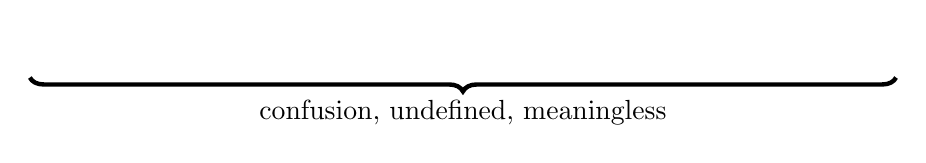
\begin{tikzpicture}
\draw [decorate,decoration={brace,amplitude=5pt,mirror,raise=4ex}, ultra thick]
  (1,0) -- (12,0) node[midway,yshift=-3em]{confusion, undefined, meaningless};
\end{tikzpicture}
}

\end{frame}

\section{Free/open science}

\begin{frame}{Free/open science}

\begin{itemize}
\item Open/free science. Popular topic nowadays.
\item Different ``definitions'', none of them very clear. Confusion.
\item Few establish some basic principles. Very few make explicit a theory of science. Confusion.
\item Under our system \textbf{a science is free if it is not subject to confusion}.
	\begin{itemize}
	\item ``Negative'' definition. Point out confusion and return to technique/science.
	\item A positive definition would be redundant since it is provided by the science itself (in its positive operation). A science is free when it proceeds according to its defined, unaltered nature.
	\end{itemize}
\end{itemize}
\end{frame}

\end{document}


